\documentclass{standalone}
\usepackage{ tikz }
\usetikzlibrary{shapes}
\usetikzlibrary{plotmarks}
\usepackage{ xparse }
\usepackage{../../../macros}

\begin{document}
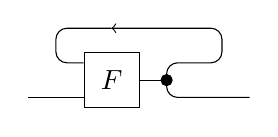
\begin{tikzpicture}[yscale=-1,x=1em,y=1.25em]
        
    \draw (-1,0) -- (1,0);
    \node[draw, minimum height = 2em, minimum width = 2em, anchor = west] at (1,-0.5){$F$};
    \draw (3,-0.5) -- (4,-0.5);
    \filldraw (4,-0.5) circle (2pt);
    \draw [rounded corners, ->] (4,-0.5) -- (4, -1) -- (6,-1) -- (6, -2) -- (2, -2);
    \draw [rounded corners] (2,-2) -- (0,-2) -- (0,-1) -- (1,-1);
    \draw [rounded corners] (4,-0.5) -- (4, 0) -- (7,0);

\end{tikzpicture}
\end{document}